\documentclass{amsart}
\usepackage[letterpaper, margin=1.25in]{geometry}
%\usepackage{etoc}
\usepackage{tikz}
\usepackage{float}
\usepackage{hyperref}

\newlength\tocrulewidth
\setlength{\tocrulewidth}{1.5pt}

\hypersetup{
	colorlinks=true,
	linkcolor=blue,
	filecolor=magenta,      
	urlcolor=cyan,
}

\usepackage{array}
\newcolumntype{P}[1]{>{\centering\arraybackslash}p{#1}}

\author{
	Kind, Matias
	\texttt{mcarras2@illinois.edu}
	\\ \and\\
	Hariri, Sahand
	\texttt{hariria2@illinois.edu}
}
\title{Isolation Forest Using Spark}

\begin{document}	
\maketitle
We consider parallelizing the isolation forest algorithm using Spark. The following are six different ways in which we can parallelize the algorithm.

The experiment is performed for a training dataset consisting of 4000 data points distributed as a two dimensional normal distribution with mean $\left[\begin{matrix}10 \\  1 \end{matrix}\right]$ and covariance $\left[\begin{matrix}1 & 0 \\  0 & 1\end{matrix}\right]$. The same data is used for computing anomaly scores for testing purposed. Figure \ref{fig:iso_forest} shows this dataset as well as the distribution of anomaly scores computed using the algorithm. We have added some anomalous points manually. 

\begin{figure}[H]
	\includegraphics[width=1\linewidth]{/Users/sahand/Research/iso_forest/report/images/iso_forest.png}
	\caption{On the left, we have the dataset. Some sample anomalous data points discovered using the algorithm are highlighted in black. We also highlight some non-anomalous points in red. On the right, we have the distribution of anomaly scores obtained by the algorithm.}
	\label{fig:iso_forest}
\end{figure}

Each case of testing is performed five times, and the mean and the variance of the time taken to perform each trial are reported in seconds in table \ref{tab:results}. 
	
	\begin{enumerate}
		\item \textbf{Case 1}: Create 800 trees in a single core and run everything serially.
		\item \textbf{Case 2}: Create 100 trees in 8 cores. Each core has access to the full data set for training purposes. For scoring, each core receives the whole data and runs it through forests of size 100. At the end the scores from each forest are aggregated. 
		\item \textbf{Case 3}: Split the data for training among 8 cores. Each core has 100 trees. Scoring is done similarly to Case 2. 
		\item \textbf{Case 4}: Split the data for training among 8 cores. Each core has 800 trees. Scoring is done similarly to the previous two cases. This naturally is expected to take the longest. 
		\item \textbf{Case 5}: 800 trees in a single core. After training, distribute the trees over the cores, and compute the scores in a vectorized way.
		\item \textbf{Case 6}: Split the data for training among 8 cores. Score each partition in one of the cores and simply collect data. 
	\end{enumerate}

\begin{table}[H]
	\caption{Summary of results.}
	\label{tab:results}
\begin{tabular}{| P{3cm} || P{2cm} | P{2cm} | P{2cm} | P{2cm} |}
	\hline
	           &\multicolumn{2}{c|}{Forest Assembly}& \multicolumn{2}{c|}{Computing Score}\\
	\hline
	           & Mean & Var & Mean & Var\\
	\hline
	 Case 1 & 3.2501 & 0.0219   & 71.4731  & 0.0559\\
	\hline
	Case 2 & 0.0063 & 1.274e-7 & 16.8996  & 0.8627\\
	\hline
	Case 3 & 0.0073 & 1.702e-6 & 21.1470  & 0.8066\\
	\hline
	Case 4 & 0.0064 & 2.886e-6 & 163.54 & 16.169\\
	\hline
	Case 5 & 6.6305 & 0.6377 & 44.616 & 6.8809\\
	\hline
	Case 6 & 0.0071 & 8.574e-7 & 3.2851 & 0.02851\\
	\hline
\end{tabular}
\end{table}

The data in the table above is summarized graphically in figure \ref{fig:TimeComparison}. Note that the y-axes are not on the same scale. 

\begin{figure}[H]
	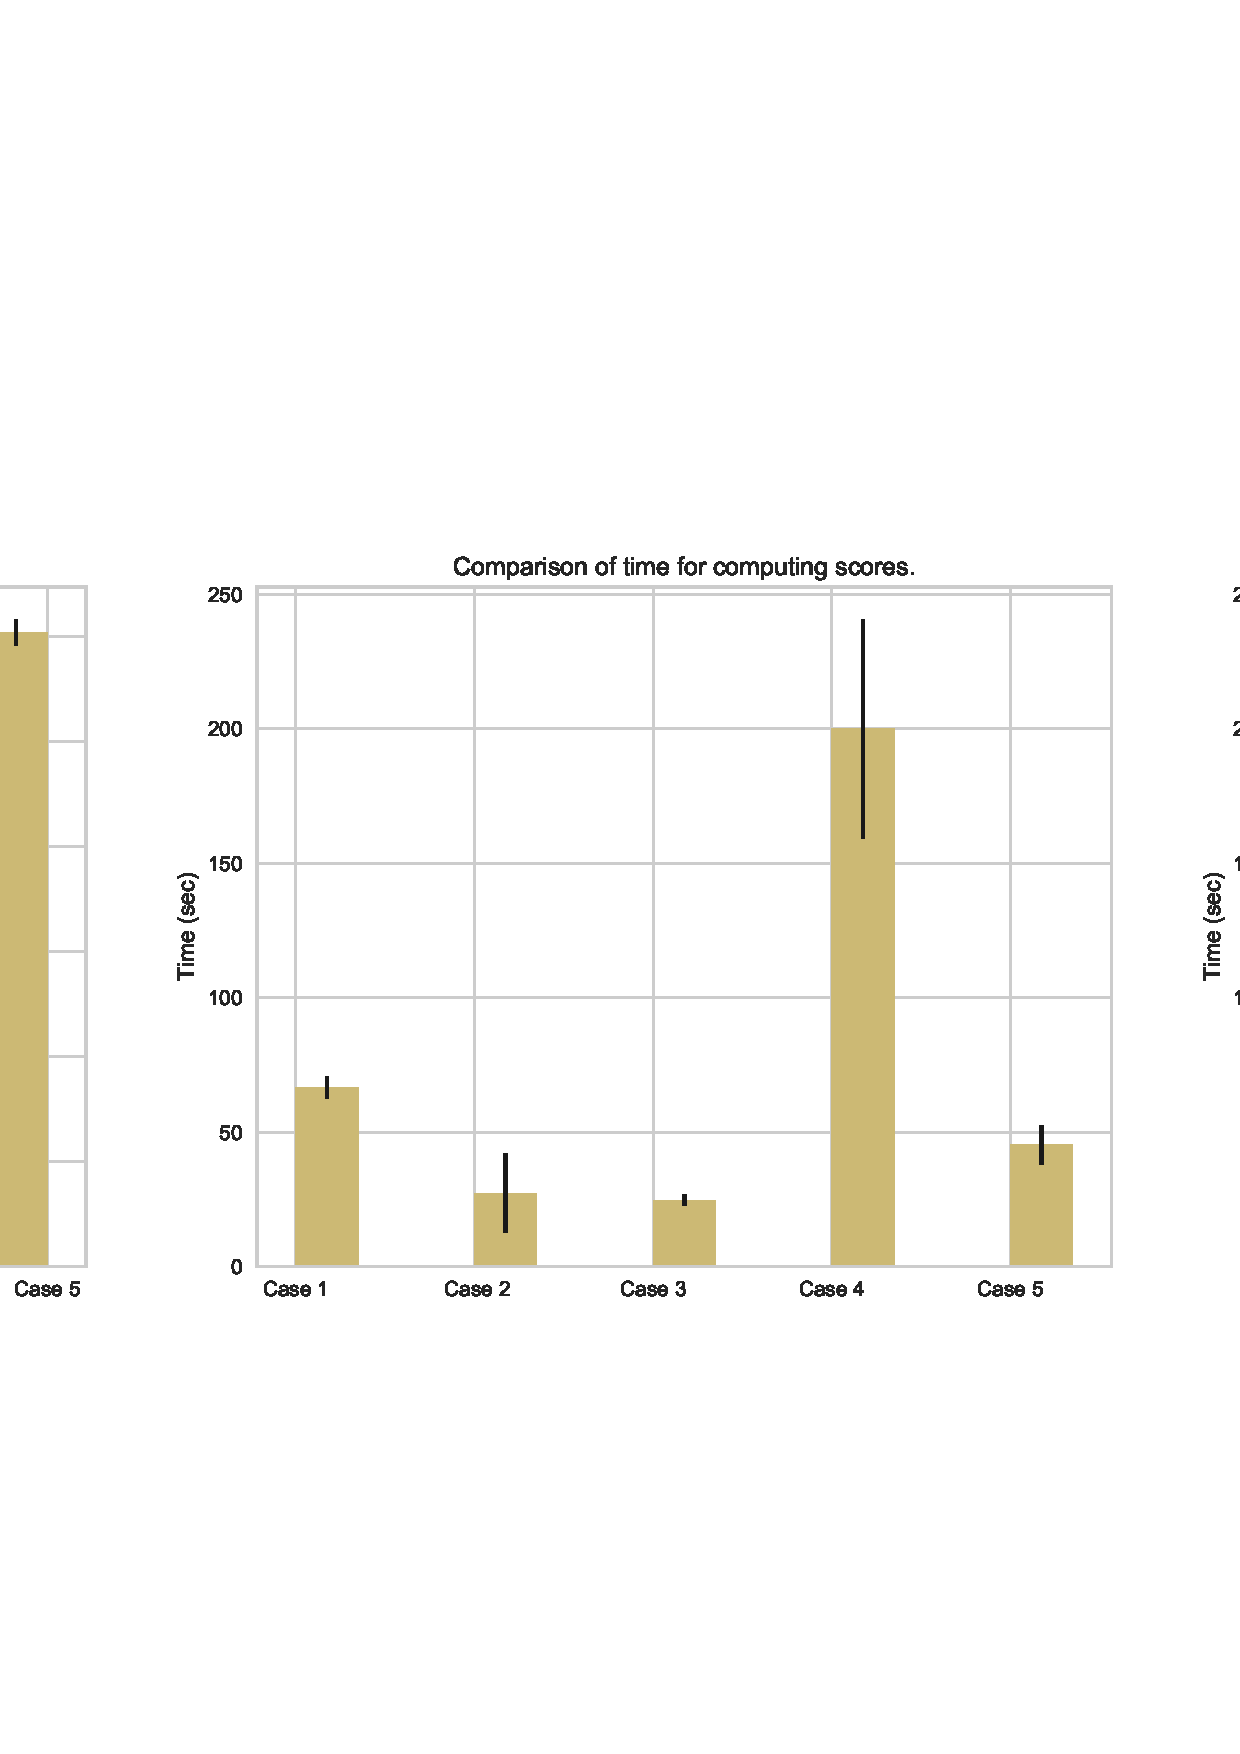
\includegraphics[width=1\linewidth]{/Users/sahand/Research/iso_forest/report/images/TimeComparison.png}
	\caption{Comparison of time taken for training and obtaining anomaly score for each case listed above. The plot on the left shows the time taken to train and distribute the trees among the cores. The plot on the right shows the times taken to compute the anomaly scores using each method.}
	\label{fig:TimeComparison}
\end{figure}

As another metric, we consider the case of running serially to be the benchmark case. We then compare the anomaly score, $S$,  for each data point obtained using each of our parallelization methods with the benchmark. The measure of the comparison is the following:

\begin{align}
	E = \frac{100}{N} \left( \sum_{i=1}^{N} \left( \frac{S^\text{parallel}_i - S^\text{benchmark}_i}{S^\text{benchmark}_i}\right)^2 \right)^\frac{1}{2}	
	\label{eq:Difference}
\end{align}
%
where $N$ is the number of data points. Figure \ref{fig:Difference} shows the value of $E$ for each case. Putting these results together with the total time taken for each case (training and scoring) shown in figure \ref{fig:TotalTime}, we can see that case 3 perhaps offers the best performance.


\begin{figure}[H]
	\includegraphics[width=1\linewidth]{/Users/sahand/Research/iso_forest/report/images/rmsdiff.png}
	\caption{Difference computed as shown in equation \ref{eq:Difference}}
	\label{fig:Difference}
\end{figure}


\begin{figure}[H]
	\includegraphics[width=1\linewidth]{/Users/sahand/Research/iso_forest/report/images/TimeComparisonTotal.png}
	\caption{Total average time taken to run each case. This includes training, distributing trees, and computing scores.}
	\label{fig:TotalTime}
\end{figure}


Another interesting thing to look at is the question of how the difference between each case and benchmark changes as the anomaly score grows. Intuitively the larger anomaly scores should also show the largest discrepancy. In order to take a look at this, we sort the data points by anomaly scores associated with them using the benchmark case, and plot the anomaly score for each in figure \ref{fig:SortedScores}.

\begin{figure}[H]
	\includegraphics[width=1\linewidth]{/Users/sahand/Research/iso_forest/report/images/SortedAnomolyScore.png}
	\caption{We sort the data points in the benchmark case according to their anomaly scores. We then sort the data points in other cases according to the position each one assumed in the benchmark case.}
	\label{fig:SortedScores}
\end{figure}

Now taking each case of this sorted list and plotting the relative difference of each case with the benchmark, we have the results shown in figure \ref{fig:SortedScoresDiff}. We can kind of see that as the anomaly score grows, the difference on average also increases in each case (case 2 looks a little shady though). 


\begin{figure}[H]
	\includegraphics[width=1\linewidth]{/Users/sahand/Research/iso_forest/report/images/SortedAnomolyScoreDiff.png}
	\caption{We now look at the square difference between data points from each case and the benchmark after sorting them.}
	\label{fig:SortedScoresDiff}
\end{figure}

Next steps:

\begin{enumerate}

	\item Get Spark up and running on a Kubernetes cluster.
	\item Run all of this on the said cluster.
	\item Think about how to train data continuously as new data comes in. 

\end{enumerate}


More to come...

\end{document}\textsl{}